 \documentclass{article}

% If you're new to LaTeX, here's some short tutorials:
% https://www.overleaf.com/learn/latex/Learn_LaTeX_in_30_minutes
% https://en.wikibooks.org/wiki/LaTeX/Basics

% Formatting
\usepackage[utf8]{inputenc}
\usepackage[margin=1in]{geometry}
\usepackage[titletoc,title]{appendix}

% Math
% https://www.overleaf.com/learn/latex/Mathematical_expressions
% https://en.wikibooks.org/wiki/LaTeX/Mathematics
\usepackage{amsmath,amsfonts,amssymb,mathtools}

% Images
% https://www.overleaf.com/learn/latex/Inserting_Images
% https://en.wikibooks.org/wiki/LaTeX/Floats,_Figures_and_Captions
\usepackage{graphicx,float}

% Tables
% https://www.overleaf.com/learn/latex/Tables
% https://en.wikibooks.org/wiki/LaTeX/Tables

% Algorithms
% https://www.overleaf.com/learn/latex/algorithms
% https://en.wikibooks.org/wiki/LaTeX/Algorithms
\usepackage[ruled,vlined]{algorithm2e}
\usepackage{algorithmic}

% Code syntax highlighting
% https://www.overleaf.com/learn/latex/Code_Highlighting_with_minted
\usepackage{minted}
\usemintedstyle{borland}

% References
% https://www.overleaf.com/learn/latex/Bibliography_management_in_LaTeX
% https://en.wikibooks.org/wiki/LaTeX/Bibliography_Management
\usepackage{biblatex}

% Indent the first paragraph of a section
\usepackage{indentfirst}

% Title content
\title{FACVC Project Proposal}
\author{Guilherme Silva\\
Faculdade de Engenharia da Universidade do Porto \\
up201603647@fe.up.pt}
\date{}

\begin{document}

\maketitle

The problem is a simplification of the biggest problem in Adaptive Optics.
This term comes from technology used in optical systems to recover angular
resolution, often called image quality. Which is lost when the observations
are made through turbulent mediums.

The solution to it lies in estimating the optical wave-fronts from measurements
and the applying its inverse to a collection of sophisticated deformable
mirrors in real time.

In this project, I aim to tackle only a simplification of the problem. Which
consists of a telescope with only four mirrors spaced in accordance with Fig.
\ref{diagram}. The data necessary is going to be simulated using the algorithm 
below:


\begin{enumerate}
    \item Randomize the position of each of the mirrors (piston, tip and tilt);
    \item Calculate the phase map for each of the mirrors;
    \item Compose the matrix of the telescope with the phases of the 4 mirrors;
    \item Calculate the electric field in each point of the telescope
          \ref{electric-field} where $\phi$ is the phase at the point and 
          $A$ is a constant;
    \item Calculate the measurement of the telescope's sensor using \ref{sensor},
          where $\hat{E}$ corresponds to a fourier transform of $E$.
\end{enumerate}

\begin{figure}[htbp]
    \centering
    
    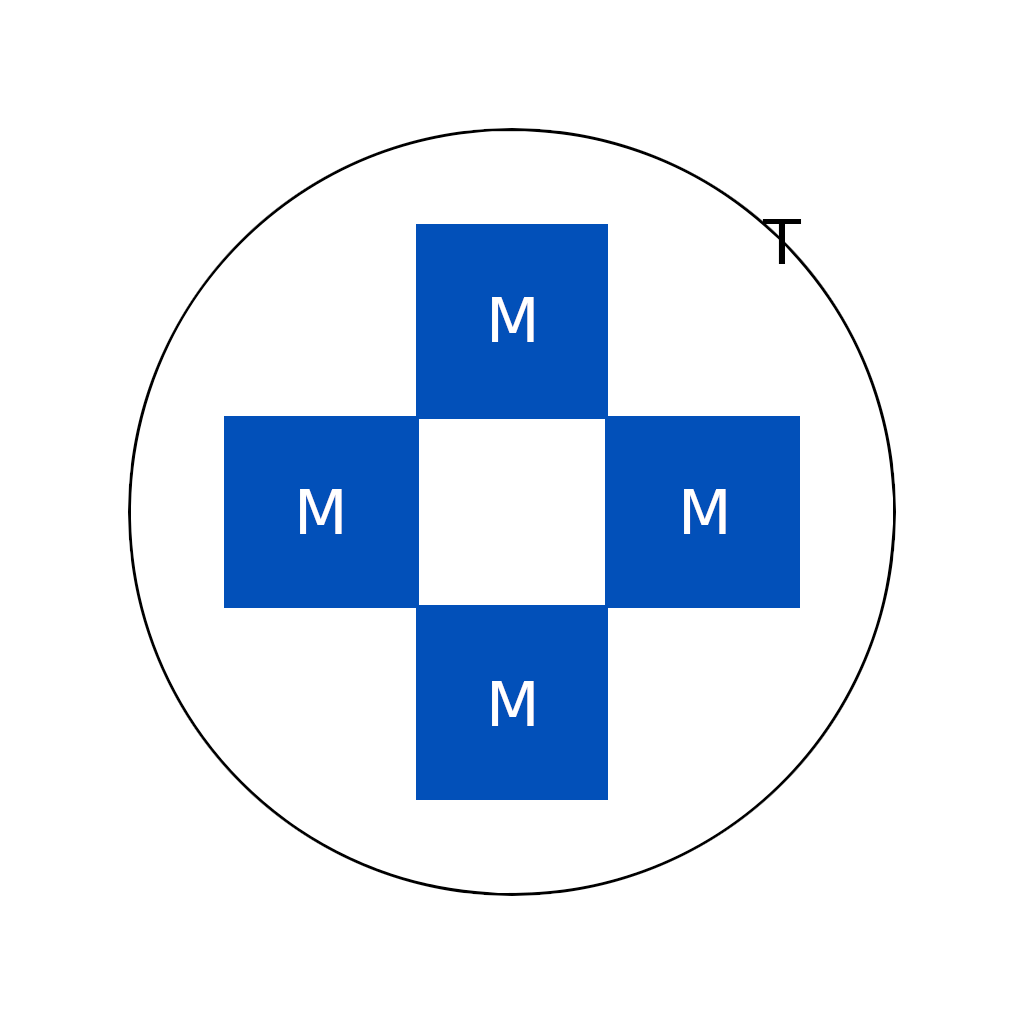
\includegraphics{telescope_diagram.png}
    \caption{Diagram of the telescope: (M): deformable mirrors, (T): telescope
    lens}
    \label{diagram}
\end{figure}

\begin{equation}\label{electric-field}
    E =  Ae^{(\imath \phi)}
\end{equation}

\begin{equation}\label{sensor}
    s = |\hat{ E }|^2
\end{equation}

After the data is generated, I aim to tackle the regressions problem of
determining the original position of the mirrors from the estimated sensor
measurements. For this I will explore deep learning algorithms such as
Convolutional Neural Networks and try to do some feature extraction to
apply more traditional methods such as Support Vector Machines.
\end{document}
